%\documentclass{sig-alternate-05-2015}
\documentclass[sigconf]{acmart}
\usepackage{url}
%\usepackage{arial}
\let\proof\relax
\let\endproof\relax
\usepackage{amsmath,amsfonts,amssymb,amsthm}
\usepackage{graphicx}
\usepackage{epsfig,multirow, color}
\usepackage{subfigure}
\usepackage{wrapfig}
\usepackage{psfrag}
\usepackage{algorithm}
\usepackage{latexsym}
\usepackage{algorithmic}

\theoremstyle{plain}
\newtheorem{thm}{Theorem}[section]
\newtheorem{lem}[thm]{Lemma}
\newtheorem{prop}[thm]{Proposition}
\newtheorem*{cor}{Corollary}


%\theoremstyle{definition}
\newtheorem{defn}{Definition}
\newtheorem{conj}{Conjecture}
\newtheorem{exmp}{Example}

\theoremstyle{remark}
\newtheorem*{rem}{Remark}
\newtheorem*{note}{Note}

%%%%%%%%%%%%%%%%%%%%%%%%%%%%%%%%%%%%%%%%%%%%%%%%%%%%%%%%%
%%%%%%%%%%%%%%%%%%%%%%%%%%%%%%%%%%%%%%%%%%%%%%%%%%%%%%%%%
%  USE THIS? (To move table caption down)
 \usepackage{caption} 
 %\captionsetup[table]{skip=5pt}
%%%%%%%%%%%%%%%%%%%%%%%%%%%%%%%%%%%%%%%%%%%%%%%%%%%%%%%%%%
%%%%%%%%%%%%%%%%%%%%%%%%%%%%%%%%%%%%%%%%%%%%%%%%%%%%%%%%%%


\usepackage{booktabs} % For formal tables
%\setcopyright{none}

\begin{document}

\title{Hardware Isolation Mechanisms for Security Improvement in FPGAs}
%
%\author{Festus Hategekimana}
%\affiliation{%
%  \institution{University of Arkansas}
%  \city{Fayetteville}
%  \state{AR}
%  \country{USA}}
%  \email{fhategek@uark.edu}
%  
%\author{Taylor JL Whitaker}
%\affiliation{%
%  \institution{University of Arkansas}
%  \city{Fayetteville}
%  \state{AR}
%  \country{USA}}
%  \email{txw043@uark.edu}   
%   
%\author{Md Jubaer Hossain Pantho}
%\affiliation{%
%  \institution{University of Arkansas}
%  \city{Fayetteville}
%  \state{AR}
%  \country{USA}}
%  \email{mpantho@uark.edu} 
%  
%\author{Christophe Bobda}
%\affiliation{%
%  \institution{University of Arkansas}
%  \city{Fayetteville}
%  \state{AR}
%  \country{USA}}
%  \email{cbobda@uark.edu}


\begin{abstract}
Field Programmable Gate Arrays (FPGAs) platform security management continues to be a strong area of concern despite recent increased adoption and integration of FPGAs into commercial scale cloud computing systems. One of the technical problems in the FPGA security management area has been the lack of hardware primitives to support multi-tenancy while enforcing proper domain isolation. In this paper, we present a tutorial on recent progress that have been made to address this issue. Specifically, we present hardware isolation mechanisms that can be used to enable domain separation on FPGAs.
\end{abstract}


\begin{CCSXML}
<ccs2012>
<concept>
<concept_id>10002978.10003001.10003003</concept_id>
<concept_desc>Security and privacy~Embedded systems security</concept_desc>
<concept_significance>500</concept_significance>
</concept>
<concept>
<concept_id>10002978.10003001.10003599</concept_id>
<concept_desc>Security and privacy~Hardware security implementation</concept_desc>
<concept_significance>500</concept_significance>
</concept>
<concept>
<concept_id>10010583.10010600.10010628.10011716</concept_id>
<concept_desc>Hardware~Reconfigurable logic applications</concept_desc>
<concept_significance>500</concept_significance>
</concept>
</ccs2012>
\end{CCSXML}

\ccsdesc[500]{Security and privacy~Embedded Systems Security}
\ccsdesc[500]{Security and privacy~Hardware Security Implementation}
\ccsdesc[500]{Hardware~Reconfigurable Logic Applications}
\keywords{FPGA Security, Hardware Isolation, IP Containerization, CAPSL
}


\maketitle


\section{INTRODUCTION}\label{sec:intro}
Many of today's critical embedded systems are increasingly relying on FPGA-based SoCs because of the useful balance between performance, scale, flexibility, and rapid
time to market they provide. This was recently exemplified with the recent Audi announcement that its 2018 A8 world's first Level 3 autonomous driving system will
feature Altera's Cyclone FPGA SoCs for object and map fusion processing tasks. It's not just in embedded systems space where we are seeing accelerated adoption of FPGA platforms. The latter are also being continuously integrated into commercial scale cloud computing systems and data centers as evidenced by Amazon recent announcement that it is providing cloud compute instances with FPGAs (EC2 F1).

FPGAs security continues to be a strong area of concern. Specifically, current FPGA platform does not possess any hardware primitives that would allow support for multi-tenancy while enforcing proper domain isolation[STILL WORKING ON INTRODUCTION]. 

\section{HARDWARE ISOLATION MECHANISMS} \label{sec:problem_definition}

This section discusses current techniques that are employed to enforce hardware isolation on FPGAs. This list is by no means exhaustive and it is beyond the scope of this paper to discuss these techniques in greater details. The interested reader is encouraged to refer to cited works.  


\subsection{Hardware-enforced Access Control Lists (FESTUS)}

In this approach, a hardware module or a microcontroller-based firmware-upgradable module is used to monitor and enforce authorized sharing of system
resources among cores. Memory-access security policies are expressed in a specialized language,and a compiler translates these policies directly to a circuit (or a microcontroller) that enforces the policies.The circuit is then loaded onto the FPGA along with other components of the system.

There are many research efforts with some relation to this approach, but to the best of our current knowledge, works in [CITATION] and in [CITATION] are the only work with similar goals that come close to ours here. In their work, they designed and implemented a reconfigurable reference monitor (RM) which implements an access control list (ACL). They then integrated the reference monitor into the on-chip peripheral bus (OPB) and used it to regulate access to the memory and peripherals. Memory and peripherals accesses go through a reconfigurable monitors access control list [3]. The access control list associates every object (memory ranges for ex.) in the system with a list of principals (IP cores) with the rights of each principal to access the object[3]. In their implementation, each object access has to be computed by the reference monitors ACL at runtime. The decision is either granted access or denied access. Since this access model can create potential memory performance issues in large memory applications, they proposed a mechanism in which a buffer is used to hold the data until the ACL grants approval of the legality of the request [3]. Figure ~\ref{fig:ted} illustrates the implementation.For example, in case of a write, the data to be written is stored in the buffer until the ACL grants the approval, at which time the write request is sent to the memory [3].


\begin{figure}[hbt]
\centering 
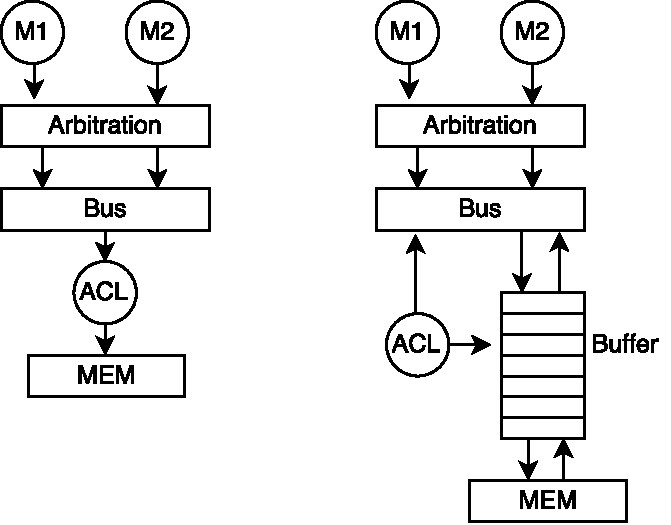
\includegraphics[width=0.75\columnwidth]{figures/ted_access.pdf} 
\caption{Access Model Implementation. On the left, there's no "caching" mechanism. On the right, a buffer is used to hold the data while access rights are being looked up.} % The text in the square bracket is the caption for the list of figures while the text in the curly brackets is the figure caption
\label{fig:ted} 
\end{figure}



Authors in [CITATION] observed that in Huffmire et al. access model implementation if you had consecutive and repeated memory access from the same ``principal" to the same ``object". Each one of these requests would still have to go through the reference monitor's computation. This can potentially create performance issues in large designs. These issues can be avoided by adding the capability to remember access decisions. Authors in [CITATION] built upon this observation and proposed an improved implementation of this architecture by adding capability to remember access decisions to allow them to be administered at run-time without re-computations. Figure ~\ref{fig:access} shows their proposed access model. 

\begin{figure}[hbt]
\centering 
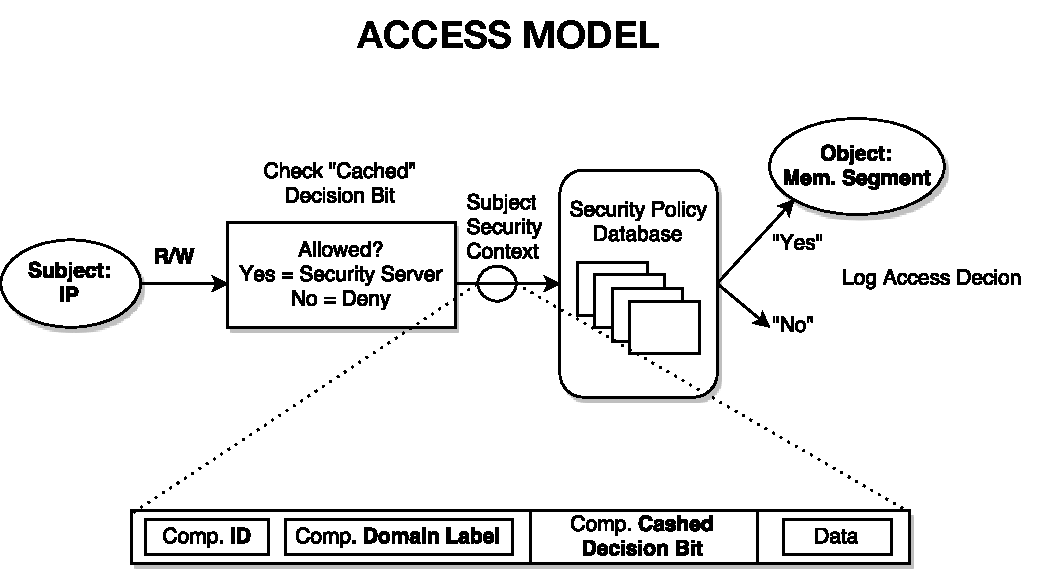
\includegraphics[width=1\columnwidth]{figures/access.pdf} 
\caption{Improved Access Model Implementation.} % The text in the square bracket is the caption for the list of figures while the text in the curly brackets is the figure caption
\label{fig:access} 
\end{figure}

Both of these techniques follow a similar design flow. Systems components are defined and implemented using hardware synthesis tools such as Xilinx's Vivado or Xilinx's XPS.  The hardware-enforced ACL core is generated by some policy compiler and it's then integrated with the rest of the system components similar to adding a standard custom IP to your design [CITAT],[CITAT]. In some instances, however, there can be compatibility issues. Sometimes standard integration of the ACL core can be complicated with the fact that sometimes some security-relevant attributes may not be directly available as parameters or easily derived from available parameters (for example, the current version of the AXI Interconnect IP core API available in Vivado 2016 does not present a component ID as a parameter). In situations like these, it's up to the application designer to build their own custom OPB (or AXI interconnect) IP which directly integrates this ACL security functionality. 

Authors in [CITATION], [CITATION] observed that the above described techniques assume a ``trusted" reference monitor to enforce the security policies and with no mechanism through which the platform itself can authenticate the authority of the reference monitor before it administers access policies decisions. The security concern here is that an attacker could conduct a man-in-the-middle attack on the system by inserting a malicious circuit inside the only authority entrusted with administrating shared resources access decisions. To mitigate this, they proposed an improved implementation of the reference monitor which combines the monitoring approach with ``proof-carrying hardware" concept. Their approach consisted of using a consumer-producer approach, where a consumer specifies a desired functionality of the memory access monitor and sends this specification to the producer and the producer synthesizes this information into a bitstream. The producer re-extracts the logic function from this bitstream and, together with the original specification, computes some miter function (which outputs an error flag if the specification and implementation differ for at least one input vector). This proof of reference monitor correctness is then generated along side with the bitstream and is sent to the consumer. The latter verifies the proof, and in case of success partially reconfigures the monitor with security policies.The consumer verifies the proof of correctness from the producer by extracting the monitor's logic function from the bitstream and forms a miter in conjunctive normal form in the same way as the producer, but with the original specification. This new miter is compared to the producer's miter and if they both match, the implementation is accepted and the monitor is accepted. The monitor is rejected if the the miters do not match. 
  

\subsection{OS-Enforced Security: Zynq FPGA TrustZone (FESTUS)}

In this approach, systems developers rely on embedded operating system to provide system security services. Security features provided include, but are not limited to confidentiality/integrity protection of the external memory containing the application code and data.

A recent example of this approach is the ARM TrustZone security architecture currently available to Zynq-7000 SoCs. In this example, the Xilinx Zynq-7000 processor
system supports ARM TrustZone technology in both the PS and PL domain.The ARM TrustZone architecture makes trusted computing within the embedded world possible by establishing a trusted platform, a hardware architecture that extends the security infrastructure throughout the system design. Instead of protecting all assets in a single dedicated hardware block, the TrustZone architecture runs specific subsections of the system either in a ``normal world" or a ``secure world." 

In the Zynq-7000 AP SoC, a normal world is defined as a hardware subset consisting of memory regions, L2 cache regions, and specific AXI devices. The Zynq-7000 AP SoC supports ARM TrustZone technology in both the PS and PL domains of the device. The PS provides a set of configuration registers related to TrustZone support for custom IPs. These configuration registers are then dynamically programmed by the software during execution. All slave IP cores instantiated in the logic can be individually assigned a Secure or Non-Secure designation. For Xilinx slave IP cores, Secure/Non-Secure configuration can be statically designated at the AXI interconnect level during system creation process. 

Figure \ref{fig:ted} shows a simplified example of how to secure your design sensitive components from illegal hardware access using Zynq-7000 AP SoC TrustZone technology

\begin{figure}[hbt]
\centering 
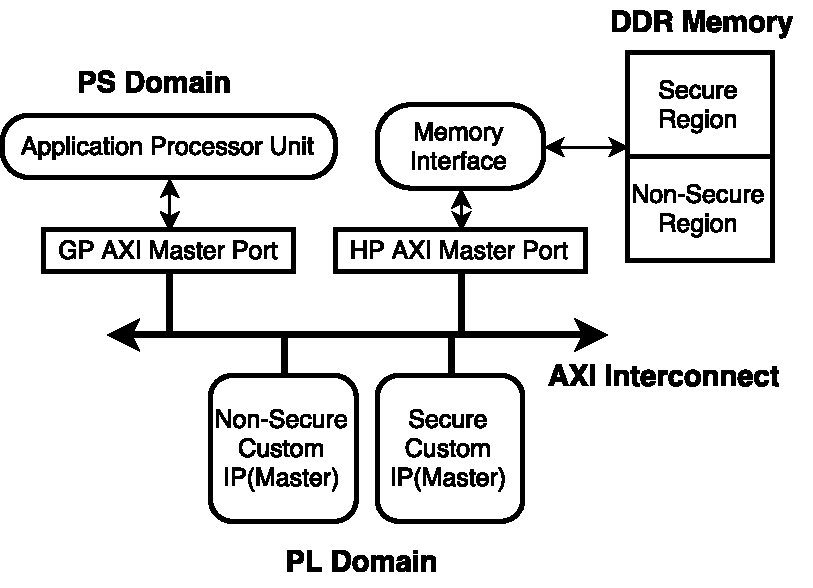
\includegraphics[width=1\columnwidth]{figures/TrustZoneHardware.pdf} 
\caption{Improved Access Model Implementation.} % The text in the square bracket is the caption for the list of figures while the text in the curly brackets is the figure caption
\label{fig:trustzone} 
\end{figure}

In this example, also available in [], on the hardware level the PL domain uses two custom master IP cores: 

\begin{itemize}
\item \textbf{Secure Custom IP:} This performs Secure read/write transactions to DDR using the HP slave port in the PS. It is also connected to the Application Processor Unit (APU) via a GP master port for register configuration.
\item \textbf{Non-Secure Custom IP:} This is used to perform read/write transactions from/to the PS DDR upon requests from the “external world.” It performs Non-Secure
read transactions to DDR using an HP slave port. Configuration of this IP is done by the PS processor through a GP master port. 
\end{itemize}

Upon power-on, the PS processor initializes both custom IPs, configures registers to establish Secure and Non-Secure regions in DDR memory, and transfers private
data/instructions to the Secure DDR region. After initialization and upon receiving a data request from the external interface, the
Non-Secure custom IP first copies the data from the external interface to the Non-Secure region of DDR memory. It then interrupts the PS processor, which
commands the Secure custom IP to perform the appropriate data computations using its private data/instructions in conjunction with the data just copied to the
Non-Secure region of DDR memory. After computation is completed, Secure custom IP puts the computed data into the Non-Secure DDR region and interrupts the PS processor to command the Non-Secure custom IP to start transferring data from the requested location.


On the software level, application processes (and their IPs) with non-secure status designation execute in memory space separated from processes with secure status designation. When a user process running in the Non-Secure world requires Secure execution, it makes a request to the Non-Secure kernel to enable the TrustZone Secure Monitor to transfer execution of the process to the Secure world. The Secure Monitor mode links the two zones and acts as a gatekeeper to manage program flow between them. 

To ensure integrity of the TrustZone software, Zynq-7000 provides a secure boot flow; where the on-chip BootROM code starts the whole security chain by ensuring that first-stage bootloader (FSBL) is signed and verified.

\subsection{CAPSL(TAYLOR)}
Our multi-layer perceptron is a supervised learning model. In machine learning, supervised learning means that model ``infers" a general function from a finite set of labelled training data \cite{regularization}. The process of inferring the weights of the neural network is called training. To check the accuracy of the neural network, error functions such as sum-squared-error (SSE), mean square error (MSE), root mean square error (RMSE) are employed. The error function most commonly used with neural networks is sum-squared-error. In our implementation, we also employed the sum squared error function to check the fitness of our neural network. Equation \ref{eq:sse} illustrates the formula to calculate sum squared error. It gives the sum of the squared error over the entire training set (size N) when the number of output dimensions is M. \begin{math}y_{ij}\end{math} is the actual output value and \begin{math}\hat{y}_{ij}\end{math} is the predicted output of the MLP

\begin{equation} \label{eq:sse}
SSE=\sum_{i=1}^{N}\sum_{j=1}^{M}(y_{ij}-\hat{y}_{ij})^2
\end{equation}

Over the years, a number of optimization methods have been developed to balance the weights and biases of the MLP: genetic algorithms, simulated annealing, hill climbing, among others. Although each one has its own advantages, the research field of machine learning steers towards one single method and its variations, for its effectiveness and scalability - gradient descent. Gradient descent is faster and easy to implement. It is a very generic optimization technique. Gradient descent is based on analytically calculating the direction to where the error function decreases the most, i. e. the negative of the derivative of the error function in relation to the weights. Equation \ref{eq:deriv_sse_1} represents this derivative at the \textit{j-th} output dimension in relation with the weight connecting the \textit{k-th} input to the neuron.

 \begin{equation} \label{eq:deriv_sse_1}
\frac{\partial SSE}{\partial w_{jk}}=\frac{\partial}{\partial w_{jk}}\sum_{i=1}^{N}(y_{ij}-\hat{y}_{ij})^2
\end{equation}

\begin{equation} \label{eq:weight_update}
w_{jk}\leftarrow w_{jk}-\eta\frac{\partial SSE}{\partial w_{jk}}
\end{equation}
With the calculated gradient, every weight can be updated by taking a step in the opposite direction. Equation \ref{eq:weight_update} provides the formula to update the weights. In stochastic gradient descent, instead of computing the gradient for the mean squared error of the whole training set, updates are applied at every instance presented to the network. This means that there is no need to sum the derivative over the entire dataset, the update can be applied at every instance presented to the network. This converts the former two equations to equations \ref{eq:deriv_se} and \ref{eq:weight_update_se}.

 \begin{equation} \label{eq:deriv_se}
\frac{\partial SE}{\partial w_{jk}}=-2(y_j-a(\mathbf{W_jx}+b))a'(\mathbf{W_jx}+b)x
\end{equation}
\begin{equation} \label{eq:weight_update_se}
w_{jk}\leftarrow w_{jk}-\eta\frac{\partial SE}{\partial w_{jk}}
\end{equation}

In our work, we adapted stochastic gradient descent (SGD) as the optimization method. The reason for choosing SGD is that 1) it works well for error manifolds with many local maxima/minima (by jerking the model out of local minima into a region that is more optimal) and 2) it is fast.  Since this analysis is true only for a neural network with a single layer, the gradient related to any weight when other layers are added can be easily calculated using a method called backpropagation. In backpropagation, error values are used to calculate the gradient of the loss function with respect to the weights in the network. Then, this gradient is fed to the optimization method, which in turn uses it to update the weights, in an attempt to minimize the loss function. In our design, we applied backpropagation to update the weights in our neural network. The activation function used in our MLP is tanh (hyperbolic tangent). The hyperbolic tangent is monotonic, evaluates to 0 at the origin, and it is differentiable. This makes it a good activation function for MLPs.

\subsection{Regularization} \label{regularization}
One of the problems faced by neural networks training procedure is overfitting \cite{overfitting}. It refers to fitting the training data too closely, making the system unable to produce reasonable outputs for those inputs not encountered during training. One way of avoiding overfitting is weight regularization. This is achieved by not allowing the weights to become too large. There are different regularization techniques that can be applied to address the overfitting problem. L1 regularization and L2 regularization are a few of these techniques. L2 regularization generates large amounts of small weights whereas in L1 regularization, sparse weights are generated. We trained our neural network with L1 and L2 regularization and compared their accuracy performance. Table \ref{tab:regularization} summarizes the results. 

\begin{table} [H] 
\centering
\caption{REGULARIZATION} \label{tab:regularization}
\begin{minipage}[b]{\linewidth}
\renewcommand{\arraystretch}{0.6}
\addtolength{\tabcolsep}{-2.7pt}
\renewcommand{\thefootnote}{\thempfootnote}
\renewcommand{\thempfootnote}{\fnsymbol{mpfootnote}}
\begin{center}
\begin{tabular}{ c | c | c | c }
%\hline
 \textbf {TYPE} & \textbf{ACCURACY} & \textbf{ERROR} & \textbf {MISSES(out of 10k)}\\
\midrule
\midrule
%\hline
\ L1    &    96.76\%  \ &    3.24\% \ & 324      \ \\
%\hline
\ L2    &    96.89\%  \ &    3.11\% \ & 311      \ \\
%\hline
\ No regularization    &    97.01\%   \ &    2.99\% \ & 299      \ \\
%\hline
\end{tabular}
\end{center}
\end{minipage}
\end{table}

As table \ref{tab:regularization} indicates, the accuracy of the system is nearly the same for all implementations. This observation lead us to choose L1 regularization as our optimization method. The reason was that even though L1 regularization suffers a few points drop in the accuracy, it has the benefit of reducing weights to near zero, if they do not contribute significantly to the neural network. By trimming the weights whose absolute value is below some threshold, we can drastically reduce the number of weights. This in terms reduce the complexity of the MLP. By avoiding the majority of the floating point operations, we can minimize burden on our small embedded processor. In L1 regularization weights are penalized according to their absolute value. Figure ~\ref{fig:regularization} illustrates this.

\begin{figure} [H]
\centering
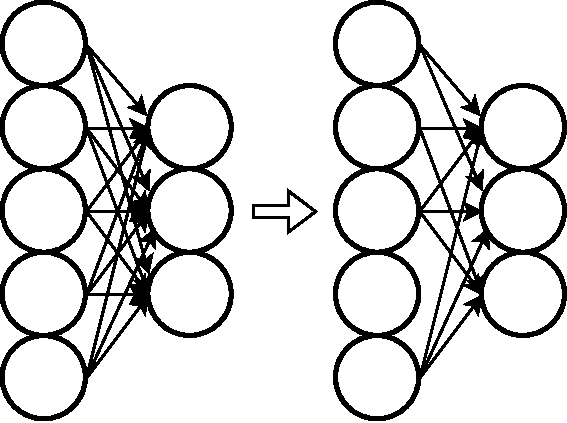
\includegraphics[width=.4\linewidth]{regularization.pdf}
\caption{Before and after L1 regularization}
\label{fig:regularization}
\end{figure}

Equation \ref{eq:weight_update_se_l1} shows the regularized update rule for the weights of the MLP. $w'$ refers to the weight after being normally updated using backpropagation, $w''$ refers to the original weight before the update and $\delta$ is the empirically chosen scaling factor. 
 
\begin{equation} \label{eq:weight_update_se_l1}
w = \begin{cases}
		w'-\delta  & \text{if } w'' \geq 0 \\
		w'+\delta & \text{if } w'' < 0
	\end{cases}
\end{equation}


\section{System Design and Implementation} \label{sec:design}

In this section, we start by discussing why a SoC design was the preferable design choice. We then discuss how we partitioned the design into software and hardware components. This is followed with a discussion on how we trained the perceptron and what the results were. The section concludes with a discussion on the prototype implementation of our design. 

\subsection{Design Motivation}

As we discussed in Section ~\ref{sec:intro}, implementation approaches which rely on back-end server computations are prone to suffer from network latency issues. A client side solution (i.e. a solution that doesn't rely on back-end server computations) which can provide acceptable detection accuracy levels within ``reasonable" detection time  is usually more desirable. FPGA SoCs are suitable for this application because of the performance and flexibility they provide.

\subsection{Design Partition}

Our proposed design is a hardware-software solution. Figure ~\ref{fig:proposed_design} illustrates our design processing flow and partitions.

\begin{figure} [H]
\centering
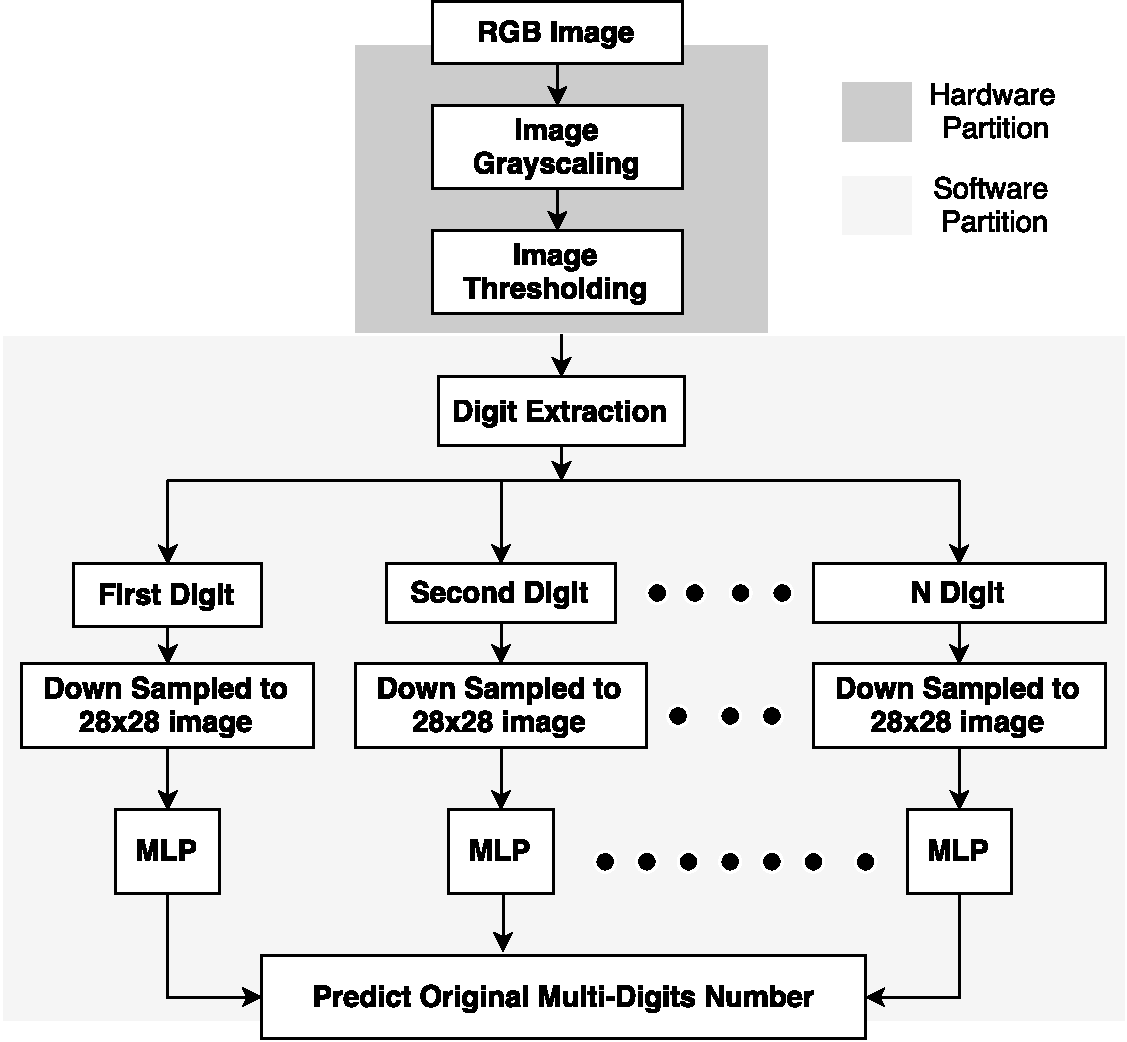
\includegraphics[width=.9\linewidth]{FPLDiagram2.pdf}
\caption{Proposed Design}
\label{fig:proposed_design}
\end{figure}

First, hand-written multi-digit numbers images in RGB (Red, Green, and Blue) format are supplied to the system through some camera input. Then, we apply grayscaling to get a monochromatic image. The reason behind this is, for this particular class of problem, the color information is not relevant as much as the luminosity. To attenuate potential illumination variances and differences in the background, we applied thresholding. The result is a binary image that we then proceed to store in the memory. This part is implemented in hardware. 

In the software portion, we first fetch the binary image from the memory. Then, we extract each individual digit from left to right. Each extracted image array is then downsampled into a 28x28, the same size of MNSIT images, binary image that we then feed into the perceptron. The latter, previously trained offline with the MNIST data set, classifies each digit and then reconstruct the original number.

\subsection{Digit Extraction Process}


First step of multi-digit prediction algorithm is to successfully extract each digit. Many of the existing methods use segmentation and complex features extraction in order to extract individual digits from the numeral string. In our work, we implemented a different and computationally efficient approach to extract digits. To detect the start of each digit, the system scans through each of the column from left to right looking for first non-zero column that indicates the start point of a digit. After detecting the starting point,  the system looks for the first all zero column in the image. This column indicates the end boundary of that digit. Within these two columns the system scans through the rows to attain the row boundaries of that hand written digit.  The pixel values between these four points are then copied to another n28xn28 (n=1,2,3...) size image. Digit in the new image is then down-sampled by n to fit in a 28x28 image. The search for the next digit starts from the previously found all zero column. Figure ~\ref{fig:digitExtract} provides a visual illustration of our digit extraction process.

\begin{figure} [hbt]
\centering
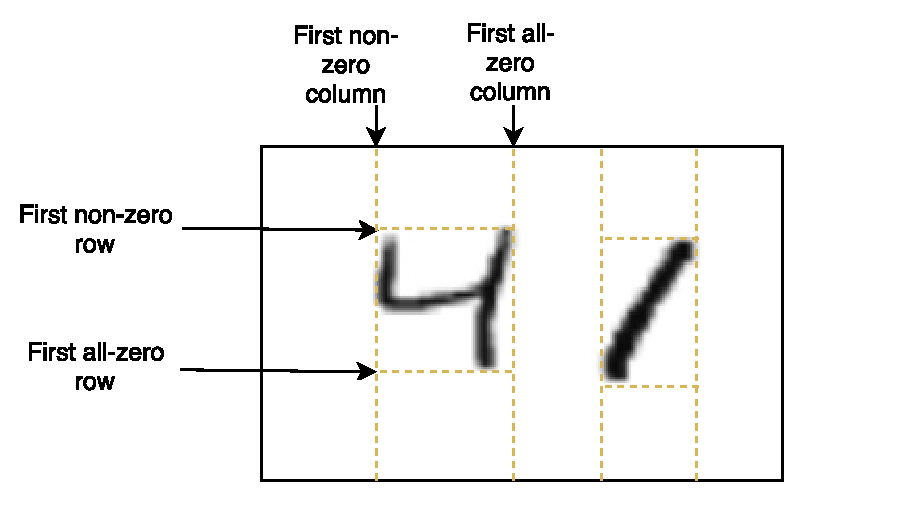
\includegraphics[width=.8\linewidth]{extract.pdf}
\caption{Visual illustration of digit extraction process}
\label{fig:digitExtract}
\end{figure}

The MNIST database we used to train our MLP was constructed from NIST's Special Database 3 and Special Database 1; which contain binary images of handwritten digits. These images were then centered in a 28x28 image by computing the center of mass of the pixels, and translating the image so as to position this point at the center of the 28x28 field. This constrained us to also map the extracted digits to the center of a 28x28 image in order to achieve good performance in our MLP.


\subsection{Digit Recognition Process}

Before we discuss the digit recognition process, let's first discuss how we trained the perceptron.

\subsubsection{Training on  MNIST Dataset}
The MNIST dataset used in this work has a training set of 60000 and a test set of 10000 handwritten digits (each has 28x28 grayscale pixels, each being represented by 8 bits) \cite{726791}. Figure \ref{fig:sampledigit} shows a random sample of this dataset. 

\begin{figure} [hbt]
\centering
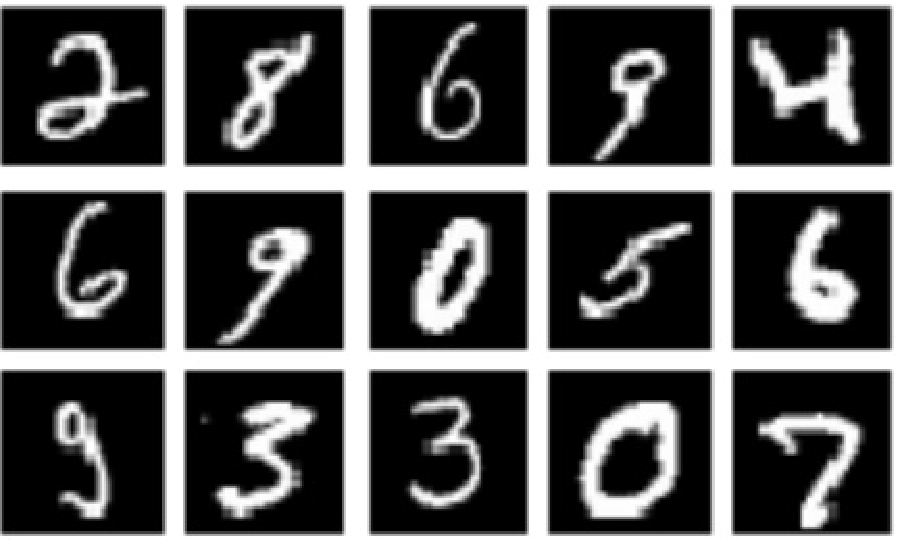
\includegraphics[width=0.5\linewidth]{MNIST_sample.pdf}
\caption{Sample MNIST digits}
\label{fig:sampledigit}
\end{figure}

As we discussed in section \ref{regularization}, the end goal of a neural network design is to obtain a network that performs well on inputs not encountered during training \cite{726791}. To achieve this, we empirically found out, through trial and error, that three layers with neurons are good enough to achieve generalization. Figure~\ref{fig:neural_net} shows the neural network model we implemented. It is a 3 layers neural network. The input layer has 300 neurons, each neuron takes 784 pixels of the handwritten digit image as input. The subsequent layers have 100 and 10 neurons, respectively. The 10 output neurons will be activated proportionally to the network prediction. 

\begin{figure} [hbt]
\centering
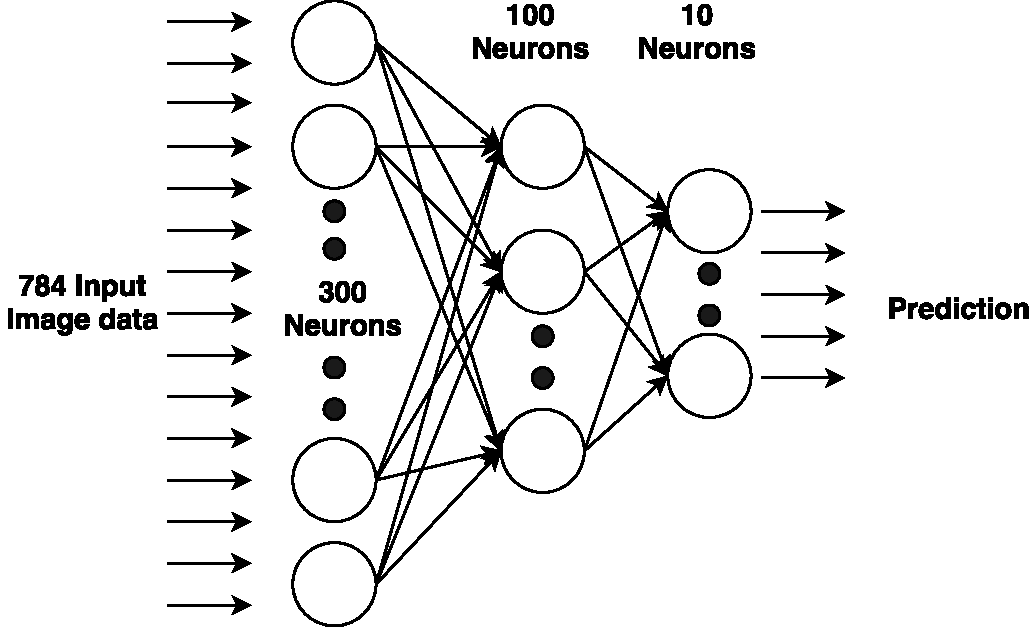
\includegraphics[width=0.85\linewidth]{neural-network.pdf}
\caption{ The implemented neural network. It consist of three layers- an input layer with 300 neurons, an output layer with 10 neurons and a hidden layer comprising 100 neurons. Each neuron in the input layer takes 784 pixels of image data. The activation function used in all the layers is hyperbolic tangent.}
\label{fig:neural_net}
\end{figure}

We trained our MLP with stochastic gradient descent and backpropagation on the 60000 instances of the training set. All input values were normalized by a division by 256. The learning rate was set to 0.01 and it decreased by a factor of 0.997 after every epoch of training. This is because if the learning rate is very small, it takes many steps to get to the optimum. However, if the learning rate is too big, it is possible to diverge instead of converge. We found that a learning rate of 0.01 was fast enough for the system to converge. The weights and bias are initialized to small random values picked from a normal distribution. The L1 regularization decay is set to 0.0001. Figure \ref{fig:misses} shows the evolution of the training procedure over each epoch. The MLP was trained on a 3.10GHz 64bit Intel® Core i5-2400 processor with 12GB RAM. The MLP best performance was found to be 324 misses out of 10000 training data, with approximately 1.2 hours training time. Although, a missing rate of 3.24\% is a few points up compared to the state-of-the art, in the context of the target application, it is still a solid performance for a client-side solution that do not rely on powerful servers and many hours of training.


\begin{figure} [hbt]
\centering
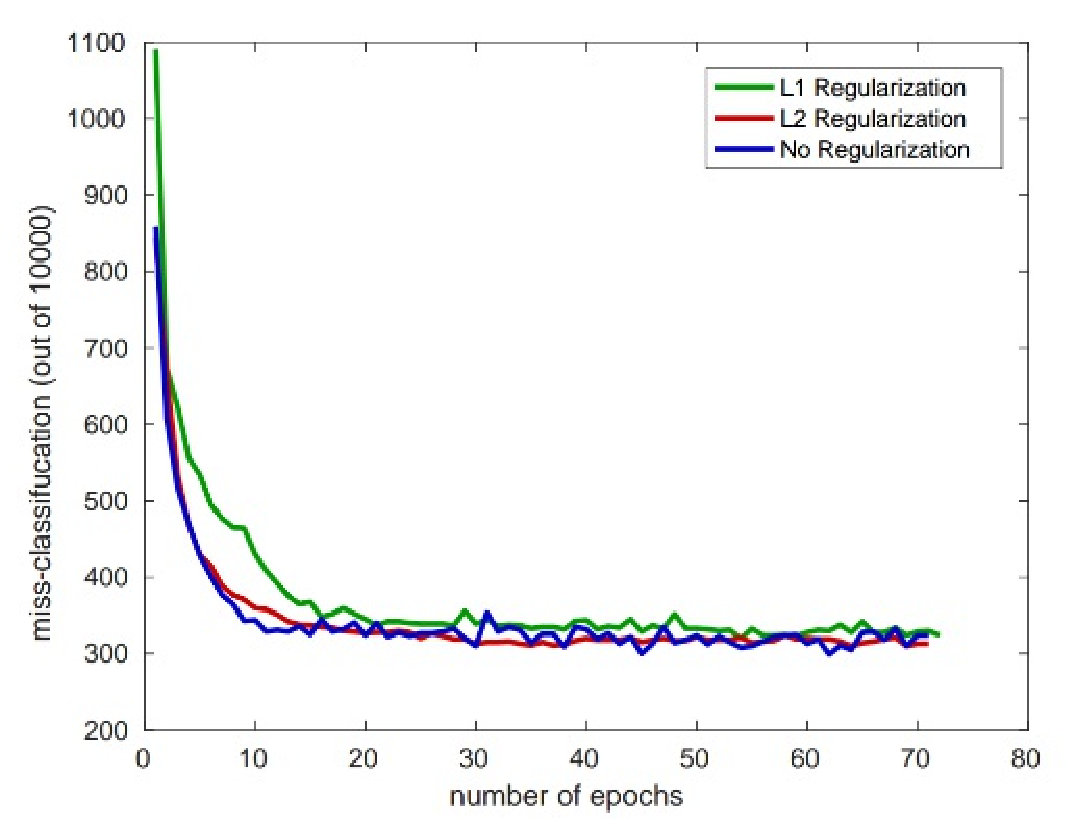
\includegraphics[width=0.85\linewidth]{misses.pdf}
\caption{MLP Training with L1 and L2 is shown. Both optimization methods are also compared to MLP training without regularization. }
\label{fig:misses}
\end{figure}

\subsection{Design Implementation}
We implemented our design on the Zybo, a development board for the Zynq MPCore FPGA. The latter is a programmable logic ( Zynq PL) coupled with a diffused 650Mhz dual-core Cortex-A9 processor (Zynq PS) \cite{xilinxzynq}. Figure \ref{fig:proposedArchitecture} illustrates our implementation. 

\begin{figure} 
\centering
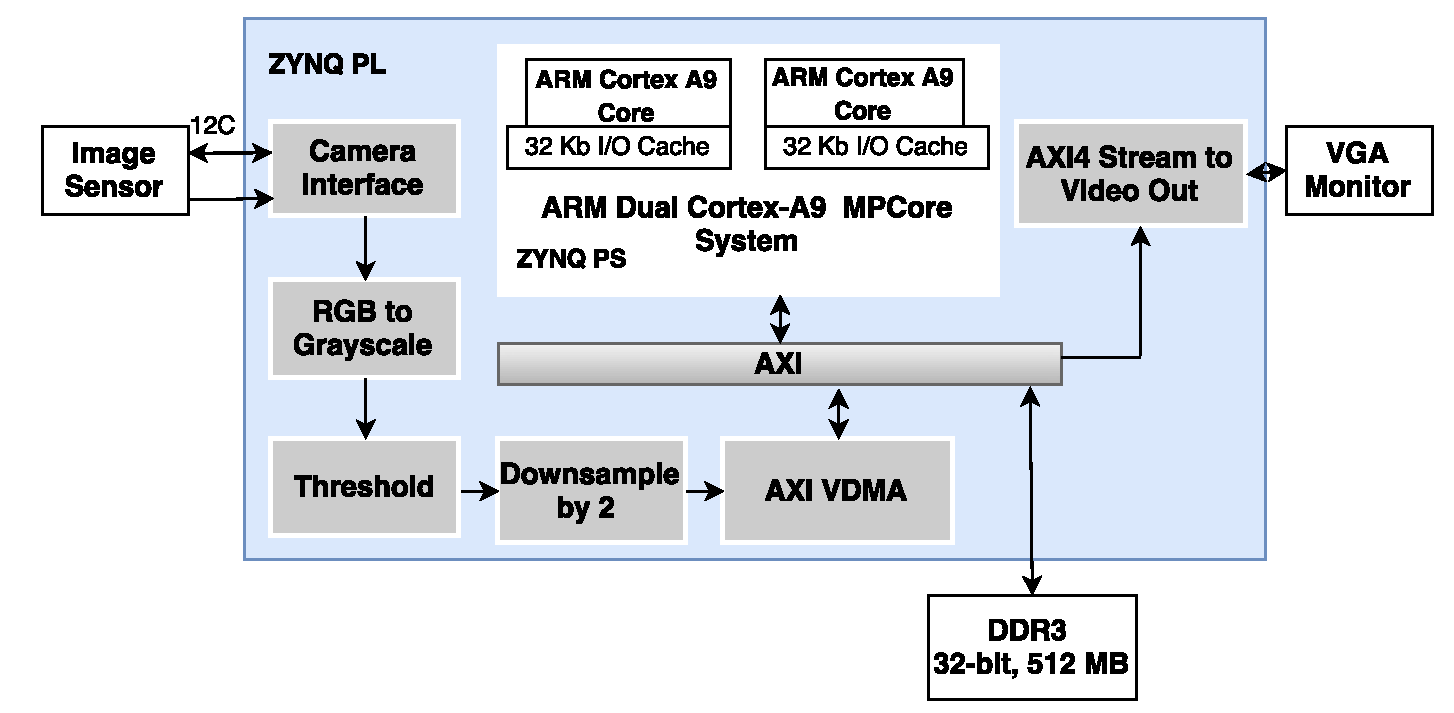
\includegraphics[width=1\linewidth]{FPLDiagram.pdf}
\caption{SoC Implementation of the hand-written digit numbers recognition system.}
\label{fig:proposedArchitecture}
\end{figure}

The application works as follow: The camera interface IP takes a 640x480 image input in RGB format from the camera. The camera used in our system is low voltage CMOS image sensor that provides full functionality of a single-chip VGA camera and image processor. Camera parameters are configured using I2C protocols. It transmits half of an 16-bit RGB (5:6:5) pixel during one pixel clock cycle. Capture block latches the first half and the second half together to produce a 16 bit RGB data. 

The RGB to-Grayscale IP takes RGB data as input and converts them into grayscale images (8-bit data). The luminosity formula to convert RGB triplets to gray-scale is traditionally $Y=0.2126R+0.7152G+0.0722B$ . In our design, in order to avoid the use of floating point operations in FPGA, we simplified the formula to $Y=0.25R+0.5G+0.12B$  where these fraction values of RGB data can easily be obtained by right shifting operations. This enabled us to obtain increased performance without losing digit extraction accuracy.

To attenuate illumination variances and differences in the background, we applied thresholding operation. The MNIST dataset is composed of bright digits written over a dark background. This means that the pen strokes have positive integer values near 255 and the background is always 0. To better approximate this scenario, The threshold IP core is used to read these grayscaled pixels and convert the image into a binary image. Equation \ref{eq:threshold} illustrates the precise operation.


\begin{equation} \label{eq:threshold}
Y' = \left\{ 
  \begin{array}{l l}
    0 & \quad \text{if $Y>T$}\\
   255-Y & \quad \text{if $Y\leq T$}
  \end{array} \right.
\end{equation} 

Following the thresholding, the binary image is then downsampled by two. This step reduces the image size from 640x480 to 320x240. The reason to do so is to reduce the amount of data transfer from PL to PS. We have seen that this downsampling of image does not degrade the performance of the MLP. Further, it means that the rest of the system will require less pixels to process. These image frames are then fed into a AXI Video DMA ipcore. This ipcore writes the image frames into the memory. We implemented the digit extraction and detection tasks on the software when we realized they were not going to fit on the device if implemented as hardware blocks.

On the software side, the Zynq processor of Zybo reads the binary image frames from the memory and extracts the digits in the right order. The extracted digits are then fed into our trained neural network for prediction. The trained weights obtained after the offline training procedure are then hard coded into C++ header files. The software part of the algorithm is written in C++ and cross compiled with GCC.
The image frames are read back from the memory using AXI4-Stream to Video Out IP core which serves to convert AXI4-Stream data into 24 bit RGB format. The latter is then formatted and sent out to the on board VGA ports for display. 

\section{Evaluation} \label{sec:results}

This section starts with a discussion on the resource utilization of our implementation. This is then followed with a discussion on how our SoC implementation performance compares to software only implementations and a discussion on the execution time analysis of our implementation. 

\subsection{Resources Overhead}


Table ~\ref{tab:resources} shows the device resources utilization and the power consumption of the designed prototype.

\begin{table} [H] 
\caption{RESOURCES UTILIZATION} \label{tab:resources}
\begin{minipage}[b]{\linewidth}
\renewcommand{\arraystretch}{0.6}
\addtolength{\tabcolsep}{-2.7pt}
\renewcommand{\thefootnote}{\thempfootnote}
\renewcommand{\thempfootnote}{\fnsymbol{mpfootnote}}
\begin{center}
\begin{tabular}{ c | c | c  }
 \textbf {RESOURCE} & \textbf{AVAILABLE} & \textbf {USAGE}\\
\midrule
\midrule
\ LUTs             &    17600      \ & 3738      \ \\
%\hline
\ LUTRAMs          &    6000       \ & 463       \ \\
%\hline
\ BRAMs            &    60         \ & 2        \ \\
%\hline
\ Dyanimc Power    &    -          \ & 1.715W    \ \\

\ Total On-Chip Power     &    -   \ & 1.851W    \ \\
\end{tabular}
\end{center}
\end{minipage}
\end{table}

\subsection{Performance}

We evaluated the performance of our SoC implementation by presenting it with random series of non-overlapping three digits and four digits numbers. Our system detected all of them. We expect our system to maintain close to 96.76\% detection accuracy as long as there's at least one all-zeroes column gap between two consecutive digits.  As part of our evaluation process, we also looked at our system's reaction time, the time it takes our system to correctly detect the numbers. The measurements were conducted on a 650MHz frequency Zynq diffused processor. Table \ref{tab:timing} summarizes the results. 

\begin{table} [H] 
\caption{PERFORMANCE OVERHEAD} \label{tab:timing}
\begin{minipage}[b]{\linewidth}
\renewcommand{\arraystretch}{0.6}
\addtolength{\tabcolsep}{-2.7pt}
\renewcommand{\thefootnote}{\thempfootnote}
\renewcommand{\thempfootnote}{\fnsymbol{mpfootnote}}
\begin{center}
\begin{tabular}{ c | c | c }
%\hline
 \textbf {TASK} & \textbf{With HW IPs} & \textbf{W/Out HW IPs} \\
\midrule
\midrule
\ Avg. extraction time/digit       &0.29 ms    &0.29 ms      \ \\
%\hline
\ Avg. prediction time/digit       &2.8 ms     &2.8 ms       \ \\
%\hline
\ Avg. execution time/digit        &2.91 ms    &7.18 ms      \ \\
%\hline
\end{tabular}
\end{center}
\end{minipage}
\end{table}


As table \ref{tab:timing} shows, the average time it take to extract and predict a digit stays the same whether this is done with software-hardware implementation or just software. The software-hardware implementation picks up speed-up gains (x2.47) from performing initial image processing operations into hardware. These initial image processing operations were important to our solution since they allowed us to avoid the use of computationally expensive approaches like segmentation to extract the digits. 



\section{Conclusion} \label{sec:conclusion}

This paper presents the first FPGA SoC implementation solution to the hand-written multi-digit numbers recognition problem. We demonstrated  a novel digit extraction method which rely on identification of images' non-zeros columns instead of the widely used computationally-expensive segmentation method, and also discussed how we employed a multi-layer neural network. The paper presents a design and an FPGA implementation of the proposed solution; and also discusses various optimization techniques in the neural network implementation that lead to increased performance. Our future work will explore the possibility of implementing the digit extraction part on the FPGA. 


\bibliographystyle{ACM-Reference-Format}
\bibliography{FPGA2018}

\end{document}